%\documentclass[runningheads,a4paper]{llncs}
\documentclass[10pt,a4paper]{article}
\usepackage[latin1]{inputenc}
\usepackage{amsmath}
\usepackage{amsfonts}
\usepackage{amssymb}
\usepackage{graphicx}
\graphicspath{ {images/} }

\usepackage{wrapfig}

\usepackage[toc,page]{appendix} % enumerating appendixes 
\newcommand{\stoptocwriting}{%
	\addtocontents{toc}{\protect\setcounter{tocdepth}{-5}}}
\newcommand{\resumetocwriting}{%
	\addtocontents{toc}{\protect\setcounter{tocdepth}{\arabic{tocdepth}}}} 

\usepackage{multicol}
\usepackage{geometry,    multirow,   amsthm, url,array}

\usepackage{tabularx}
\usepackage{longtable,booktabs}% my add-on  

\setlength{\parskip}{0.8ex}
\usepackage{xcolor}
\newcommand\myworries[1]{\textcolor{red}{#1}}
% Generated by GrindEQ Word-to-LaTeX 2007 
% LaTeX/AMS-LaTeX

%%% remove comment delimiter ('%') and specify encoding parameter if required,
%%% see TeX documentation for additional info (cp1252-Western,cp1251-Cyrillic)
%\usepackage[cp1252]{inputenc}

%%% remove comment delimiter ('%') and select language if required
%\usepackage[english,spanish]{babel}

%\usepackage{amssymb}
%\usepackage{amsmath}

%%% remove comment delimiter ('%') and select graphics package
%%% for DVI output:
%\usepackage[dvips]{graphicx}
%%% or for PDF output:
%\usepackage[pdftex]{graphicx}
%%% or for old LaTeX compilers:
%\usepackage[dvips]{graphics}


\usepackage{colortbl}
\usepackage{xcolor}

\newlength\mylength
\newcolumntype{C}[1]{>{\centering\arraybackslash}p{#1}} % centering cels in longtables

\usepackage{chngcntr} % number of sections include ssections
\counterwithin{table}{section}% table  include number of sectionn
\counterwithin{figure}{section}% figure   include number of section

\numberwithin{equation}{section} % equation   include number of section

% bibliography
\usepackage{biblatex} %Imports biblatex package
\addbibresource{references.bib} %Import the bibliography file

%charts
\usepackage{pgfplots}
% end charts

%breake url lines in bibliography
\usepackage{url}
\usepackage{breakurl} 
\usepackage[breaklinks]{hyperref}
%end  breake url lines in bibliography

%Theorem-like
% Загрузка пакет hyperref
\usepackage{hyperref}
\hypersetup{
	colorlinks=true, %set true if you want colored links
	linktoc=all,     %set to all if you want both sections and subsections linked
	% % %     linkcolor=blue,  %choose some color if you want links to tand out
	linkcolor=blue,
	filecolor=magenta,      
	urlcolor=cyan,
}
\usepackage{enumitem}
\makeatletter
\def\namedlabel#1#2{\begingroup
	#2%
	\def\@currentlabel{#2}%
	\phantomsection\label{#1}\endgroup
}
\makeatother
\theoremstyle{plain}
\newtheorem{thm}{Theorem}[section]
\newtheorem{lem}[thm]{Lemma}
\newtheorem{prop}[thm]{Proposition}
\newtheorem{cor}{Corollary}[section]

\theoremstyle{definition}
\newtheorem{defn}{Definition}[subsection]
\newtheorem{conj}{Conjecture}[section]
\newtheorem{exmp}{Example}[section]

\theoremstyle{remark}
\newtheorem*{rem}{Remark}
\newtheorem{note}{Note}[section]
% end Theorem-like

% Переносы математики.
\begingroup
\catcode`\+\active\gdef+{\mathchar8235\nobreak\discretionary{}{\usefont{OT1}{cmr}{m}{n}\char43}{}}
\catcode`\-\active\gdef-{\mathchar8704\nobreak\discretionary{}{\usefont{OMS}{cmsy}{m}{n}\char0}{}}
\catcode`\=\active\gdef={\mathchar12349\nobreak\discretionary{}{\usefont{OT1}{cmr}{m}{n}\char61}{}}
\catcode`\<\active\gdef<{\mathchar"313C\nobreak\discretionary{}{\usefont{OML}{cmm}{m}{n}\char60}{}}
\catcode`\>\active\gdef>{\mathchar"313E\nobreak\discretionary{}{\usefont{OML}{cmm}{m}{n}\char62}{}}
\endgroup
\def\times{\mathchar8706\nobreak\discretionary{}{\usefont{OMS}{cmsy}{m}{n}\char2}{}}
\def\subset{\mathchar"321A\nobreak\discretionary{}{\usefont{OMS}{cmsy}{m}{n}\char26}{}}
%\supset,\subseteq,\notin
\def\supset{\mathchar"321B\nobreak\discretionary{}{\usefont{OMS}{cmsy}{m}{n}\char27}{}}
\def\subseteq{\mathchar"3212\nobreak\discretionary{}{\usefont{OMS}{cmsy}{m}{n}\char18}{}}
\def\neq{\not=\nobreak\discretionary{}{\usefont{OMS}{cmsy}{m}{n}\char54\usefont{OT1}{cmr}{m}{n}\char61}{}}
\def\sim{\mathchar"3218\nobreak\discretionary{}{\usefont{OMS}{cmsy}{m}{n}\char24}{}}
\def\in{\mathchar"3232\nobreak\discretionary{}{\usefont{OMS}{cmsy}{m}{n}\char50}{}}
\def\to{\mathchar"3221\nobreak\discretionary{}{\usefont{OMS}{cmsy}{m}{n}\char33}{}}
\def\?#1{#1\nobreak\discretionary{}{\hbox{$\mathsurround=0pt #1$}}{}}
% Конец переносов математики.


\date{}
\raggedbottom
\begin{document}
	\begin{figure}[htbp]
	%[trim=2cm 24.2cm 13.1cm 2.2cm, clip=true, totalheight=0.105\textheight, angle=0]
		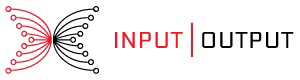
\includegraphics  {iohk-share-logo.jpg}
	\end{figure}
	
	\leavevmode \\ 
	{\Large\textbf{ Comparison of Block Expectation Time for Various Consensus Algorithms }}\\[0,5cm]
	\hrule height 0,1cm \leavevmode \\ 
	
	%	\skip
	\leavevmode \\ 
	{	\small{March 22 \textsuperscript{nd} 2017}}\\ 
	\leavevmode \\ 
	
	\begin{figure}[htbp]
		
		\begin{subfigure} %{0.3\textwidth}
			
	%		\includegraphics [scale=0.3]{etc2.png}
		\end{subfigure}
		\hfill
		\begin{subfigure} %{0.3\textwidth}
	%		\includegraphics [scale=0.2]{creative_commons.jpg}
		\end{subfigure}
	\end{figure}
	
	%	\leavevmode \\[0,5cm] 
	%{\textbf{The Veritas Team}}\\[0,5cm]
	%\leavevmode \\[0,5cm]
	
	%	\skip
	
	\leavevmode \\[0,5cm] 
	{\textbf{The Veritas Team}\\ 
		\\ 
		Dmytro Kaidalov, Lyudmila Kovalchuk, Andrii Nastenko,\\ Mariia Rodinko, Oleksiy Shevtsov, Roman Oliynykov
		\\  
		\\ IOHK.io }\\[0,5cm]
	\leavevmode \\[0,5cm]
	%	\skip
	
	
	%\maketitle
	
	%	\skip
	
	\begin{abstract}
	The blockchain technology emerged in 2008 with Bitcoin appearance. Its main technical innovation is a decentralized consensus mechanism that allows to maintain an uncensored public ledger of transactions hence giving users security guarantees that the data in a ledger can not be modified or reverted in any way. In this paper we examine typical double-spend attacks on the different blockchain-based systems and compare resulting probabilities for each of them. In our research we considered classical Bitcoin-like proof-of-work protocol, the GHOST protocol and recently introduced proof-of-stake algorithm called Ouroboros.
	\end{abstract}
	
	
	\begin{flushleft}
		\eject 
		
	\end{flushleft}
	
	
	\tableofcontents
	
	\begin{flushleft}
		\eject 
		
	\end{flushleft}
	
	\section{Introduction}
	The Bitcoin is a payment system where digitally signed transactions are grouped into blocks and stored securely in a structure called blockchain. A blockchain is a sequence of blocks linked via hash pointers where each new block contains a hash of the previous block. This structure preserves an ordered list of transactions that uniquely determines state of the system.
	
	Unlike other centralized payment systems, in Bitcoin, once a transaction is added to the blockchain it could not be considered as confirmed immediately. A user need to wait some time to be sure that the transaction is set in stone in the blockchain. This is because of decentralized nature of the system where everyone can add blocks to the blockchain. To guarantee consistency among different users and to preserve inability to revert previously added blocks, a special mechanism is used called proof-of-work. The following idea underlies a proof-of-work system: a computational effort (calculation of a hash value below some target) should be spend to produce a block. Only a chain of blocks with the most computations is considered valid.
	
	As the blockchain technology evolves the alternatives to the computationally heavy proof-of-work mechanism appear. The one most promising is called proof-of-stake: it does not require heavy computations to produce blocks, instead, a block producer is chosen through a fair procedure among all stakeholders in the system. The Ouroboros is a good example of such a system \cite{KRDO16}. To the best of our knowledge it is the first provably secure proof-of-stake protocol with rigorous security guarantees.
	
	The concept of a blockchain could be undermined if someone would have a possibility to revert blocks by submitting a chain that would substitute the one currently accepted. For example, it can lead to the following attack: some buyer pays to a merchant with bitcoins, after the corresponding transaction is included into the blockchain the merchant accepts a payment and sends a product to the buyer, upon receiving the product the buyer issues a conflicting chain of blocks which does not contain the payment to the merchant but instead sends coins back to the buyer. So as long as the merchant can not be sure that the payment is irreversible it is insecure to deliver the product.
	
	Satoshi Nakomoto argues in the original Bitcoin white paper \cite{N08} that the system is secure (with some probability) against such attacks unless 50\% or more of the total computational power possessed by an adversary.
	
	The described double-spend attack is relevant not only for Bitcoin, but also for other proof-of-work systems, for instance, those based on GHOST algorithm \cite{ZS13}, as well as for proof-of-stake systems, like Ouroboros. In this paper we describe known double-spend models for Bitcoin and present new mathematical models for the Ouroboros protocol that allows to calculate the security bounds for different types of adversaries. We also provide the results of splitting attack simulations for Bitcoin and GHOST algorithms. Finally, we compare different protocols, as a measure we focus on the block confirmation time needed to provide reasonable security guarantees for the users. 
	
	The paper is structured in the following way: the second chapter describes classical double-spend attack for Bitcoin as it was introduced by S. Nakomoto. The third chapter describes splitting attacks that are relevant to those proof-of-work systems where the time difference between blocks is not negligible compared to the block propagation time. The fourth chapter represents two adversarial models for Ouroboros proof-of-stake protocol. The last chapter summarizes and compares results from the previous chapters. 
	 
	
	\section{Double-Spend Attack: General Overview} \label{double-spend-attack-general-overview}
	
	This section represents an overview of a double-spend attack that could happen in a blockchain-based system \cite{bitcoinwiki}. As we briefly mentioned before, it does not really matter what type of consensus mechanism underlies the system, a double-spend could happen in both proof-of-work and proof-of-stake systems. Here we describe the main essence of the attack.
	
	As it follows from the name, the whole idea of a double-spend attack is to use the same coins twice. In general, it implies that someone pays for some goods, but after receiving them, reverts the payment so both goods and money are in the hands of an attacker. While it is infeasible to change the transaction with the payment itself (cause that would require falsifying a digital signature), it is possible to reject an entire block which includes the transaction. For doing this an attacker needs to substitute a valid sub-chain of blocks with a new one that has a bigger score (score calculation depends on the actual blockchain type). Even though this attack requires tremendous resources (computational in the case of proof-of-work or financial in the case of proof-of-stake system) it could be profitable.
	
	The attack involves next steps:
	\begin{enumerate}
        \item An adversary \(A\) wants to buy some goods from a merchant \(B\). For doing this, \(A\) creates a transaction \(tx_1\) with a payment to \(B\) and sends it to the blockchain (Fig. \ref{fig:Fig1}).
        \item \(B\) receives the payment from \(A\), he waits sufficient number of confirmations in the blockchain and then sends goods to \(A\) (Fig. \ref{fig:Fig2}).
        \item \(A\) creates a conflicting transaction \(tx_2\) where he redirects coins to his address and tries to generate a forked block containing this transaction. Given that \(B\) waits additional confirmations on top of the block with the payment, \(A\) needs to overcome all those blocks in his chain and create a fork with a higher score (Fig. \ref{fig:Fig3}).
        \item If \(A\) is lucky to produce a fork of the main chain, the transaction \(tx_1\) would be removed from the blockchain. Instead, the transaction \(tx_2\) would be included. The network will continue with the chain of the adversary so the payment for the merchant \(B\) would be lost forever (Fig. \ref{fig:Fig4}). At the same time the adversary \(A\) seizes both goods and money.
    \end{enumerate}
    
    \begin{figure}[h]
            \centering
            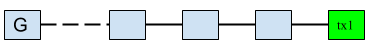
\includegraphics[width=0.4\textwidth]{Fig1}
            \caption{Initial state of the blockchain from the genesis block \(G\). The transaction \(tx_1\) is just included in the utmost block.}
            \label{fig:Fig1}
    \end{figure}
    \begin{figure}[h]
            \centering
            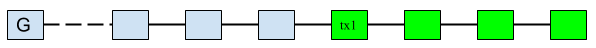
\includegraphics[width=0.6\textwidth]{Fig2}
            \caption{Merchant \(B\) waits for 3 more blocks on top of the block with \(tx_1\) and sends goods to \(A\).}
            \label{fig:Fig2}
    \end{figure}
    \begin{figure}[h]
            \centering
            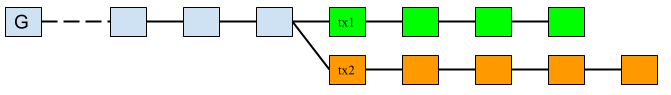
\includegraphics[width=0.7\textwidth]{Fig3}
            \caption{An adversary creates a fork with higher score.}
            \label{fig:Fig3}
    \end{figure}
    \begin{figure}[h]
            \centering
            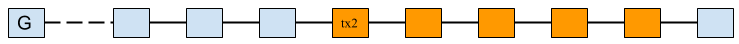
\includegraphics[width=0.78\textwidth]{Fig4}
            \caption{The network continues with the chain of an adversary. \(tx_1\) is substituted with \(tx_2\).}
            \label{fig:Fig4}
    \end{figure}
    
    Even though an exact techniques of a fork creation could varies for different consensus protocols, the essence of the described attack remains the same for all of them. 
	
	\section{Bitcoin Double-Spend Attack} \label{sec:bitcoin_models}
	
	In this section we give an overview of the existed mathematical models of the Bitcoin double-spend attack. The first one was introduced by S. Nakomoto in the original Bitcoin white paper \cite{N08}. M. Rosenfeld continued research of the Nakomoto's model and improved it in \cite{R14}. We also look into two models proposed by C. Pinzon et al. \cite{PR16} that introduce a notion of time advantage to the original model that was analyzed by Nakomoto and Rosenfeld.
	
	Worth noting that presented theoretical models for the double-spend attack could also be applied to another Bitcoin-like proof-of-work systems.
	
	\subsection{The Model of S. Nakomoto} \label{sec:nakomoto}
	
	S. Nakomoto considers the scenario when an adversary tries to generate secretly an alternate chain that would be longer (in terms of computational difficulty) than the honest chain. The race between the adversarial and honest chains is characterized as Binomial Random Walk.
	
	Given that an adversary starts with some deficit \(K\) (the honest chain is longer than adversarial on \(K\) blocks), the probability that an adversary would ever catching up with the honest chain is analogous to the Gambler's Ruin problem and could be calculated as follows:
	\[ q_K = 
	    \left \{
            \begin{tabular}{cc}
                1       & \(if\  p \leq q\) \\
                \((q/p)^K\) & \(if\  p > q\) \\
            \end{tabular}
        \right \},
	\]
	where
	
	\(p\) -- fraction of hashing power that is possessed by honest nodes (equivalent to the probability that an honest node finds next block);
	
	\(q\) -- fraction of adversarial hashing power (equivalent to the probability that an adversary finds next block);
	
	\(q_K\) -- probability that an adversary would ever catch up from the deficit of \(K\) blocks.
	
	Assuming that an adversary starts to work on malicious fork right after the payment transaction is included into the blockchain (so do not wait for \(z\) blocks after which it is confirmed by the merchant), he may have mined some number of blocks so the deficit \(K\) is reduced. The adversarial progress will be a Poisson distribution with the expected value \( \lambda = z\frac{q}{p} \).
	
	The overall probability of the successful double-spend attack can be found by multiplying the Poisson density for each possible amount of progress by the probability of catching up from the remaining deficit:
	\begin{equation} \label{eq:nak_DS}
	    DS_N(q,z) =
	    \sum_{k=0}^{\infty} \frac{\lambda^k e^{-\lambda}}{k!} \cdot
	    \left \{
            \begin{tabular}{cc}
                \((q/p)^{z-k}\) & \(if\  k \leq z\) \\
                1       & \(if\  k > z\) \\
            \end{tabular}
        \right \}
        =
        1 - \sum_{k=0}^{z} \frac{\lambda^k e^{-\lambda}}{k!}(1 - (q/p)^{z-k}).
	\end{equation}
	
	More detailed explanation of this model can be found in the original paper \cite{N08}. 
	
	\subsection{The Model of M. Rosenfeld} \label{sec:rosenfeld}
	
	Another well-known mathematical model for the Bitcoin double-spend attack, except those presented by Nakomoto, is the model of M. Rosenfeld. In \cite{R14} he clarifies and expands the work of S. Nakomoto. The same basic model is taken: for a successful double-spend attack an adversary needs to catch up from \(z = n - m\) blocks where \(n\) is the number of confirmations that a user waits before sending goods and \(m\) is the number of blocks that an adversary is expected to mine during the confirmation period.  
	
	The author considers the catching-up process as a Markov chain, where each step is defined as finding a block by the honest node or adversary:
	\[ z_{i+1} = 
	    \left \{
            \begin{tabular}{cc}
                z_i + 1 & with probability p, \\
                z_i - 1 & with probability q. \\
            \end{tabular}
        \right \)
	\]
	
	The attack succeeds if \(z\) ever reaches \(-1\). Let denote by \(\alpha_z\) the probability that an adversary would be able to catch up when he is \(z\) blocks behind. If \(z < 0\) then \(\alpha_z = 1\), otherwise \[\alpha_z = p\alpha_{z+1} + q\alpha_{z-1},\] where \(q\) is a fraction of hashing power possessed by the adversary (equivalent to the probability that he will find next block) and \(p = 1 - q\).
	
	In this case the probability to catch up with \(z\) blocks can be defined as follows:

    \begin{equation} \label{eq:ros_catchup} 
	    \alpha_z = min(q/p,1)^{max(z+1,0)} =
	    \left \{
            \begin{tabular}{ll}
                1 & \(if\  z < 0\ or\ q > p\), \\
                \((q/p)^{z+1}\) & \(if\ z \geq 0\ and\ q \leq p\).
            \end{tabular}
        \right.
	\end{equation}
	
	Similar to the model of S. Nakomoto it is possible that an adversary mines some number of blocks while the merchant waits for \(n\) confirmations in the honest chain. Recall that S. Nakomoto considers the progress of an adversary in this case as a Poisson distribution with expected value \(n\frac{q}{p}\). M. Rosenfeld took another assumption, he models the progress as a negative binomial distribution. The probability that an adversary will mine a given number of blocks \(m\) is 
	\begin{equation} \label{eq:ros_progress}
	    P(m) = \binom{m+n-1}{m}p^n q^m. 
	\end{equation}
	
	It follows that the probability of a successful double-spend attack where a merchant waits for \(n\) confirmations and an adversary succeeds to find \(m+1\) blocks during the confirmation period is equal to
	\begin{equation}  \label{eq:ros_DS}
	    DS_R(q,n) = \sum_{m=0}^{\infty}P(m)\alpha_{n-m-1} = 
	    \left \{
            \begin{tabular}{cc}
                1 - \sum_{m=0}^{n}\binom{m+n-1}{m}(p^n q^m - p^m q^n)   & \(if\  q < p\), \\
                1 & \(if\  q \geq p\). \\
            \end{tabular}
        \right.
	\end{equation}
	
	An interested reader could find more rigorous description of this model in the original paper \cite{R14}.
	
	\subsection{Other Models}
	
	It is worth mentioning two theoretical models that was presented by C. Pinzon et al. \cite{PR16}.
	
	The first one generalizes the model of M. Rosenfeld by adding an extra parameter that represents the time-advantage of an adversary. 
	
	The second one, which is called "time-based model", is completely different from those described in the previous sections. In this model the length of the valid and adversarial chains are assumed to be equal. Instead, authors are focused on the time parameter \(t\) that represents the time difference between the \(n^{th}\) block in both the adversarial and honest chains.
	
	As far as these models are consistent with the model of M. Rosenfeld and give almost the same results, we do not examine them deeply. Short descriptions are given in the Appendix \ref{sec:generalized-model} and \ref{sec:time-based-model}.
	
	\subsection{Models Comparison}
	
	Since all considered models are aimed to estimate the probability of the same double-spend attack in Bitcoin, the results are similar except differences between the models of S. Nakomoto and others. The models of M. Rosenfeld and C. Pinzon et al. give exactly similar results (assuming that the time advantage in the models of C. Pinzon is equal to zero).
	
	The table \ref{tbl:bitcoin_comparison} shows the values computed for different models. It represents the number of blocks that a user should wait to be 99.9\% sure that his transaction would not be reverted by an adversary.
	\begin{table}[h!]
        \label{tbl:bitcoin_comparison}
        \centering
    \begin{tabular}{|p{2cm}||p{2cm}|p{2cm}|p{2cm}|}
         \hline 
         Adversarial hashing power & The model of S. Nakomoto & The model of M. Rosenfeld & The model of C. Pinzon (generalized) \\
         \hline
         0.1   & 5  & 6     & 5 \\
         0.15  & 8  & 9     & 8 \\
         0.2   & 11 & 19    & 12 \\
         0.25  & 15 & 20    & 19 \\
         0.3   & 24 & 32    & 32 \\
         0.35  & 42 & 58    & 58 \\
         0.4   & 89 & 133   & 134 \\
         0.45  &    & 539   & 541 \\
         0.46  &    & 844   & 846 \\
         0.47  &    & 1502  & 1505 \\
         0.48  &    & 3382  & 3387 \\
         0.49  &    & 13533 & 13544 \\
         \hline
    \end{tabular}
    \caption{The number of blocks that a user should wait to be 99.9\% sure that his transaction would not be reverted by an adversary with the given hashing power.}
    \end{table}
	
	\section{Blockchain Splitting Attacks}
	
	This section provides a description of a splitting attack that was described in \cite{KP15}. It could be considered as a variation of a double-spend attack since the main goal is to create a fork of the required length. The splitting attack is targeted on the proof-of-work based protocols with a short block generation time that is comparable to the block propagation time in the network.
	
	We will start with a general overview of a splitting attack and then provide some experimental results showing the possibility of its application to different proof-of-work consensus protocols.  
	
	\subsection{Splitting Attack: General Overview}
	
	In contrast to classic double-spend attack described in section \ref{double-spend-attack-general-overview}, where an adversary is supposed to create a fork secretly and publish it only when it is needed, the splitting attack is public for all nodes from the beginning. Moreover, not only an adversary contributes blocks into the forked branch but also honest nodes.
	
	The idea of the attack is the following: when a fork of depth 1 accidentally happens, an adversary splits its hashing power on both branches to keep their lengths\footnotemark \ equal as long as possible. In this case honest miners would also be split due to their arbitrary chose between branches of equal lengths. When honest miners publish a new block on the one of the branches, an adversary publishes block on the other branch to keep the fork running (see Fig. \ref{fig:split}). If branches are of the same length, then adversary does nothing so again honest miners are split in half.
	
	\footnotetext{In the most proof-of-work protocols the actual criterion for branch selection is the branch difficulty, i.e., the winning branch is the one that required the most computations to create. For simplicity and because it is usually the case in a real world, it is assumed that all blocks have the same difficulty so the longest chain would be the most difficult one.}
	
	\begin{figure}[h]
            \centering
            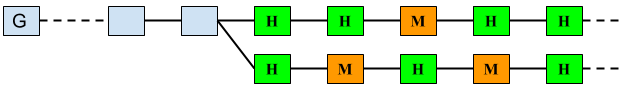
\includegraphics[width=0.75\textwidth]{split}
            \caption{The fork that keeps running while adversary is able to equalize the lengths of both branches with malicious blocks (marked with M).}
            \label{fig:split}
    \end{figure}
	
	So an adversary tries to keep both chains balanced by their length. If lengths differs, an adversary extends the chain, that is behind, by publishing some amount of blocks needed to equalize lengths of both chains. The attack continues till adversary has sufficient amount of blocks for each chain in his reserves. If he can't equalize chains lengths at the end of some round, then the attack is finished.
	
	A notion of a round was initially taken from \cite{GKL15}, it represents a complete round of information propagation to all nodes in a p2p network. In practice information propagation is a random variable with an order of tens of seconds. In the described model it is assumed that one full communication round takes 12.6 seconds (this is the average block propagation time in Bitcoin network \cite{DW13}).
	
	A general essence of the splitting attack is the following: when the time of block generation is comparable to the time of block propagation then the probability of generation 2 or more blocks in the same round (and at the same block height) becomes non-negligible. In this case, at the beginning of the next round the network would be split into two branches. An adversary leverages such block collisions to keep the fork running.
	
	Thus, an important parameter that facilitates a splitting attack is the number of POW solutions (mined blocks) per complete round of information propagation. In \cite{KP15}, where this parameter is designated as \(f\), it was shown that when \(f\) decreases and gets closer to 0, then the probability of a splitting attack decreases too (an adversary needs almost 50\% of the hashing power to make a split). And vice versa, when \(f\) increases, the security bound becomes worse (the attack becomes feasible with less than 50\% of the hashing power). The splitting attack is the most effective when \(f \geq 1 \), i.e., at the rate of 1 block per round or more.

    It follows that a short block generation time (relative to the block propagation time) creates favorable conditions for a splitting attack to occur. Hence, it becomes interesting to investigate resistance of proof-of-work protocols with different values of the parameter \(f\). In our experiments we take two most widespread protocols: Bitcoin and GHOST. Further sections represent experimental results obtained during the computational modeling for both protocols.
	
	\subsection{Bitcoin Splitting Attack}
	
	As it is known, the average block generation time in Bitcoin is equal to 10 minutes \cite{N08}. Given that the average block propagation time is 12.6 seconds \cite{DW13}, the parameter \(f=\frac{12.6}{10\cdot60}=0.021\). In what follows it is more suitable to use the parameter \(k\) instead of \(f\) that shows an average amount of communication rounds between 2 consecutive blocks: \(k=\frac{1}{f}\).
	It is interesting to estimate the possibility of a successful splitting attack for the original chose \(k=47.6\) made in Bitcoin and see how the security degrades in the case when \(k\) decreases. To accomplish this we do an experimental analysis on the described attack.
	
	The results of the simulations are summarized in Fig. \ref{fig:btc_split_chart}. It is shown what fork length an adversary can maintain with the probability of success at least 0.1\%. It is easy to see that when the time between blocks decreases an adversary gets a chance to create longer fork. 
	
	Our simulation shows that for the chose of \(k=47.6\) (like in Bitcoin) 6 confirmations are needed to be sure that the probability of a splitting attack is less than 0.1\% (considering an adversary that possesses 35\% of the hashing power). If we assume that the average block generation time is equal to the block propagation time (so that \(k=1\)) then 9 confirmation is needed for the same level of security.   
	
	\begin{figure}[h]
        \centering
        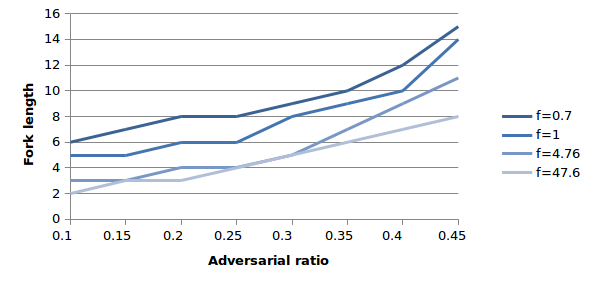
\includegraphics[width=0.75\textwidth]{btc_split_chart}
        \caption{The fork length that an adversary with a given hashing power can create with the probability of success at least 0.1\%. Different lines represents different chose of the parameter \(k\).}
        \label{fig:btc_split_chart}
    \end{figure}
	
	
	\subsection{GHOST Splitting Attack}
	
	In this chapter we first briefly describe the GHOST algorithm itself and then continue with the splitting attack application.
	
	\subsubsection{GHOST Overview}
	
    The GHOST (Greedy Heaviest-Observed Sub-Tree) protocol was initially proposed as an improvement of the Bitcoin protocol that allows to reduce the time between blocks while preserving the same level of security \cite{ZS13, ZS15}.
    
    The main modification that was suggested is that blocks that are not included in the main chain can still contribute to a chain's irreversibility. The basic observation behind the protocol is that the blocks that are built on top of some block \(B\) add additional weight to block \(B\) even if they are not in the main chain. So, in contrast to the Bitcoin protocol, where only the blocks that are in the main chain contributes to the difficulty of this chain, in GHOST a whole sub-tree of blocks is considered (Fig. \ref{fig:btc_vs_ghost}). More information in \cite{ZS13,ZS15}.
    
    \begin{figure}[h!]
        \centering
        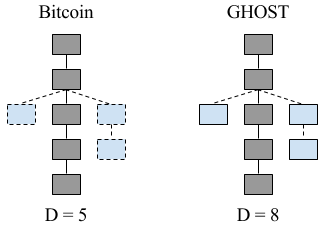
\includegraphics[width=0.4\textwidth]{btc_vs_ghost}
        \caption{The calculation of the chain's difficulty \(D\) is shown for the Bitcoin and GHOST protocols. As it could be seen, in GHOST, even the blocks that are not included in the main chain add weight to it.}
        \label{fig:btc_vs_ghost}
    \end{figure}
	
	Since it is declared by the authors that the GHOST protocol has a comparable security even with short block generation time (it is stated that even when blocks are issued every second the security level is the same as in the original Bitcoin protocol \cite{ZS13}), it becomes interesting to investigate resistance of the GHOST protocol against splitting attack.
	
	\subsubsection{Splitting Attack}
	
	The splitting attack for the GHOST protocol is slightly different compared to Bitcoin \cite{KP15}. There are two differences:
	\begin{enumerate}
    	\item An adversary has to compensate the difference in the total number of honestly mined blocks on both branches at the end of each round, while in Bitcoin-like protocols he has to compensate only the maximal number of honestly mined blocks to keep both chains balanced.
    	\item All blocks produced by an adversary are always valid. This facilitates an attack for adversary, because he can just mine the first nodes after the common prefix of the two branches. In contrast, in Bitcoin an adversary has to extend only the head of diverging chains, so all blocks must be recent. 
	\end{enumerate}
	
	The results of the simulation (Fig. \ref{fig:ghost_split_chart}) show that the attack is extremely effective when the parameter \(k\) is near to 1.
	
	\begin{figure}[h] 
        \centering
        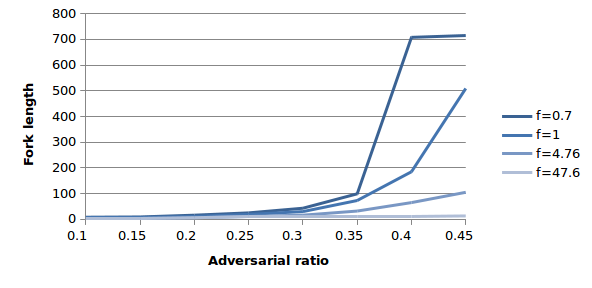
\includegraphics[width=0.75\textwidth]{ghost_split_chart}
        \caption{The fork length that an adversary with a given hashing power can create for the GHOST protocol with the probability of success at least 0.1\%. Different lines represents different chose of the parameter \(k\).}
        \label{fig:ghost_split_chart}
    \end{figure}
	
	\section{Ouroboros Double-Spend Attacks}
	
	This section provides the analysis of the Ouroboros protocol. As stated in \cite{KRDO16} it is the first provably secure proof-of-stake blockchain protocol with rigorous security guarantees, comparable to those achieved by the Bitcoin blockchain protocol.
	First we briefly discuss the protocol itself and then present two models for different types of adversaries.
	
	\subsection{General overview}
	
	As previously stated, the Ouroboros is a proof-of-stake protocol, thus it does not require heavy computations for block production. While in the proof-of-work protocols like Bitcoin the blocks are produced by the miners (which are not necessarily have a stake in the system), in Ouroboros only the stakeholders can produce blocks. Given that the stakeholders are well incentivized to keep the overall stability of the system (as it would consequently keep the value of their coins), it creates an additional incentive for block producers to act honestly, thus making a system more secure in general. 
	
	The main idea behind the protocol is that the time is divided into so called epochs, each epoch consists of predefined number of slots. Each slot has an associated stakeholder that should produce a block during the time of that slot. The model requires a synchrony among stakeholders, the blocks that are produced in the incorrect timeslots are considered invalid. At most one block could be produced in the given slot (Fig. \ref{fig:ouroboros_general}).
	
	The owners of the slots are chosen randomly before the beginning of the epoch. A randomness for a selection procedure is generated collectively by a set of stakeholders using special cryptographic protocol based on the PVSS scheme (Publicly Verifiable Secret Sharing \cite{S99}).
	
	\begin{figure}[h] 
        \centering
        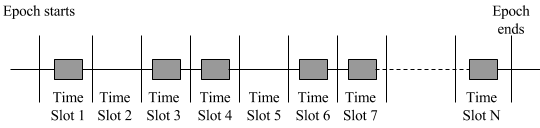
\includegraphics[width=0.75\textwidth]{Ouroboros_general}
        \caption{A general scheme of the Ouroboros protocol. The time is divided into slots, each slot has an associated stakeholder who should produce a block in this slot. It is not necessary that the block in the given slot will be produced (for instance, a corresponding stakeholder could be offline at the moment), but there is a strict rule that only one block can be produced in the slot.}
        \label{fig:ouroboros_general}
    \end{figure}
    
    \subsection{The attacks on the common prefix}
    
    Following the terminology given in \cite{KRDO16} the attack that consists in a fork creation is called an attack on a common prefix. There are two possible models for an adversary that is going to create a fork: the one that immediately discovers an adversarial behaviour and the one that leaves an adversary covert. We will briefly describe both of them.
    
    Despite of the rule that a slot winner can produce only one block per slot in the given chain of blocks, nothing can prevent him from creating several blocks in the same slot but on the different chains, thus creating a fork (see Fig. \ref{fig:ouroboros_split_attack}). An adversary can facilitate an attack by publishing blocks in both chains forcing the honest slot winners to be split between them. In what follows we will call such an adversary as general adversary.
    \begin{figure}[h] 
        \centering
        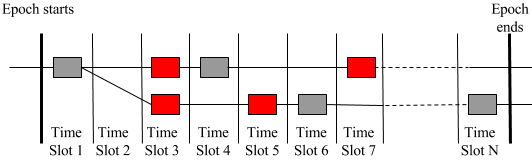
\includegraphics[width=0.75\textwidth]{ouroboros_split_attack}
        \caption{An adversary that possesses some slots (depicted in red) tries to split honest slot winners on two chains, thus facilitating an attack.}
        \label{fig:ouroboros_split_attack}
    \end{figure}
    
    While the described attack provides an adversary significant opportunities it leaves a suspicions "audit trail" - multiple signed blocks at the same slot, which immediately discovers malicious behaviour. This motivates to consider a restricted class of covert adversaries, who produce not more than one block per slot (though not necessarily in the expected slot \cite{KRDO16}).
    
    An interested reader could find more details in \cite{KRDO16, RMKQ17}.
    
    \subsubsection{General adversary} \label{sec:general_adv}
    
     A central point of the security arguments given in \cite{KRDO16} is the notions of the \textit{characteristic} and \textit{forkable strings}. A \textit{characteristic string} is a binary string \(\{0,1\}^n\) where each element indicates a slot that is assigned either to adversary (denoted with 1) or to honest user (denoted with 0). A \textit{forkable string} is a characteristic string with such disposition of adversarial slots that allows fork creation. 
     
     Understanding density of the forkable strings among all characteristic strings will help to determine the probability of an attack. In \cite{KRDO16} an upper bound on the probability of a string being forkable is given. In our research we are interested in the exact probabilities of forks. To obtain such probabilities we utilize recursive algorithm that detects a forkable string (see lemma 4.18 in \cite{KRDO16} for more details):
     
     \begin{equation} \label{eq:forkable_string}
     \begin{tabular}{l}
        m(w1) = (\lambda(w)+1, \mu(w)+1),\ and  \\[0.1cm]
        m(w0) = 
        \left \{
            \begin{tabular}{ll}
                (\lambda(w)-1,0)         & if \lambda(w) > \mu(w)=0 \\
                (0,\mu(w)-1)             & if \lambda(w) = 0 \\
                (\lambda(w)-1,\mu(w)-1)  & otherwise,
            \end{tabular}
        \right \)
     \end{tabular}
     \end{equation}
     where 
     
     \(w\) - characteristic string;
     
     \(m(w) = (\lambda, \mu)\) - a state of the string \(w\) represented by two variables \(\lambda\) and \(\mu\);
     
     \(m(\epsilon) = (0,0)\) - initial state of the algorithm.
     
     Given a characteristic string \(w\) and initial state \(m(\epsilon\)), the state is updated sequentially with each element of the string. Finally, when all elements from \(w\) are processed, the variable \(\mu\) is checked: if \(\mu \geq 0\) then the string \(w\) is forkable, otherwise it is not.
     
     Having such an algorithm it is possible to calculate the overall probability of a fork for a string of particular length. It could be done by constructing a matrix of probabilities of all possible states (Fig. \ref{matrix_fork_strings}). 
    
     \begin{figure}[h!]
        \label{matrix_fork_strings}
        \centering
        \begin{tabular}{|p{0.75cm}|p{0.75cm}|p{0.75cm}|p{0.75cm}|p{0.75cm}|p{0.75cm}|p{0.75cm}|p{0.75cm}|p{0.75cm}|}
             \hline
             \(p^{(n)}_{0,-n}\) & ... & \(p^{(n)}_{0,-2}\) & \(p^{(n)}_{0,-1}\) & \(p^{(n)}_{0,0}\) & \(p^{(n)}_{0,1}\) & \(p^{(n)}_{0,2}\) & ... & \(p^{(n)}_{0,n}\) \\
             \hline
             \(p^{(n)}_{1,-n}\) & ... & \(p^{(n)}_{1,-2}\) & \(p^{(n)}_{1,-1}\) & \(p^{(n)}_{1,0}\) & \(p^{(n)}_{1,1}\) & \(p^{(n)}_{1,2}\) & ... & \(p^{(n)}_{1,n}\) \\
             \hline
             \(p^{(n)}_{2,-n}\) & ... & \(p^{(n)}_{2,-2}\) & \(p^{(n)}_{2,-1}\) & \(p^{(n)}_{2,0}\) & \(p^{(n)}_{2,1}\) & \(p^{(n)}_{2,2}\) & ... & \(p^{(n)}_{2,n}\) \\
             \hline
             ...          & ... & ...          & ...          & ...         & ...         & ...         & ... & ...         \\
             \hline
             \(p^{(n)}_{n,-n}\) & ... & \(p^{(n)}_{n,-2}\) & \(p^{(n)}_{n,-1}\) & \(p^{(n)}_{n,0}\) & \(p^{(n)}_{n,1}\) & \(p^{(n)}_{n,2}\) & ... & \(p^{(n)}_{n,n}\) \\
             \hline
        \end{tabular}
        \caption{The matrix shows the probabilities of a random characteristic string \(w\) of length \(n\) turns out in state \(m(w)=(i,j)\). It is indexed by all possible \(\lambda\) and \(\mu\) values that could be reach by the string of length \(n\).}
    \end{figure}
    
    The matrix could be calculated iteratively using the following rules (based on the algorithm \ref{eq:forkable_string}):
     \[\begin{tabular}{l}
        p^{0}_{0,0} = 1\ and\ p^{0}_{i,j} = 0,\ for\ i \neq 0\ or\ j \neq 0, \\[0.2cm] 
        p^{n}_{i,j} = lam1\cdot q\cdot p^{n-1}_{i-1,j-1} + mu1 (1-q)p^{n-1}_{i+1,j+1} + mu2(1-q)p^{n-1}_{i+1,0} + lam2(1-q)p^{n-1}_{0,j+1}, \\[0.2cm]
        lam1 = 
        \left \{
            \begin{tabular}{ll}
                1 & if \(i > 0\), \\
                0 & otherwise;
            \end{tabular}
        \right \)
        lam2 = 
        \left \{
            \begin{tabular}{ll}
                1 & if \(i = 0\), \\
                0 & otherwise;
            \end{tabular}
        \right \) \\[0.1cm]
        mu1 = 
        \left \{
            \begin{tabular}{ll}
                1 & if \(j \neq 0\), \\
                0 & otherwise;
            \end{tabular}
        \right \)
        mu2 = 
        \left \{
            \begin{tabular}{ll}
                1 & if \(j = 0\), \\
                0 & otherwise.
            \end{tabular}
        \right \)
     \end{tabular}\]
     where \(q\) is a fraction of the adversarial stake.
     
     Finally, the probability that an adversary with \(q\) fraction of stake would be able to create a fork of \(n\) slots could be defined as follows:
     \begin{equation} \label{eq:fork_prob}
         DS(q,n) = \sum_{i=0}^{n}{\sum_{j=0}^{n}{p_{i,j}^{(n)}}}.
     \end{equation}
     
     Note that it is also possible to estimate the probability of a fork by simulating an attack directly. It could be done by generating random binary strings (taking into account the probability of adversarial slot) and checking them with algorithm \ref{eq:forkable_string}. The results are conforms to those obtained analytically with equation \ref{eq:fork_prob}.
     
    %  The equation \ref{eq:fork_prob} allows to calculate the probability of a fork of exactly \(n\) slots. But it is possible that an adversary that does not have sufficient number of slots at the moment of the slot \(n\) will be able to obtain deficient slots in the future. The eq. \ref{eq:fork_prob} could be easily expanded to accommodate this assumption:
     
    %  \myworries{TODO: The catch-up function C(q,n,k) seems to be incorrect.}
    %  \begin{equation} \label{eq:fork_prob_full}
    %      DS(q,n)_{full} = DS(q,n) + \sum_{k=1}^{n}{P(n,-k)C(q,n,k)}
    %  \end{equation}
    %  where
     
    %  \(P(n,m) = \sum_{i=0}^{n}{p_{i,m}^{(n)}}\) - the probability that after \(n\) slots an adversary would have a deficit of exactly \(m\) slots (it is a summation of the \(m^{th}\) column in matrix \ref{matrix_fork_strings});
     
    %  \(C(q,n,k) = (1 - \sum_{i=0}^{\infty}{(1 - DS(q,n+k+i))})\) - the probability to catch up from the deficit of \(k\) slots.
     
    %  In theory, an adversary can be trying to catch-up infinitely, but in practice, with each new slot, the probability decreases exponentially, thus quickly goes down to negligible values.
     
    \subsubsection{Covert Adversary} \label{sec:covert_adv}
    
    As previously stated, a covert adversary tries to keep an attack in secret until he creates a branch of sufficient length. In this case, adversarial behaviour would be to refrain from publishing blocks in the honest chain (Fig. \ref{fig:covert_adv}). 
    \begin{figure}[h] 
        \centering
        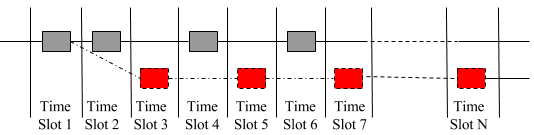
\includegraphics[width=0.75\textwidth]{covert_adv}
        \caption{A covert adversary tries to accumulate sufficient amount of slots (depicted in red) to overcome an honest chain at some moment in future.}
        \label{fig:covert_adv}
    \end{figure}
    
    In the classical double-spend attack it is assumed that an adversary has to create a fork of at least \(n\) blocks where \(n\) is the number of confirmations that a user waits before sending goods or providing service. In this formulation the attack with a covert adversary is basically close to the Bitcoin double-spend attack (see section \ref{double-spend-attack-general-overview}). Therefore, the probability of a fork after \(n\) blocks could be easily calculated using, for instance, the model of S. Nakomoto (see section \ref{sec:nakomoto}, eq. \ref{eq:nak_DS}).
    
    Because of the deterministic nature of the block creation process in the Ouroboros protocol, it is more convenient to consider the security bounds as the number of slots that a user should wait to be sure (to some degree) that a fork can not be created (opposite to the number of blocks in the classical model).
    
    In our model, for a successful attack an adversary needs to create a fork of \(l\) slots (or longer). To do this he needs to possess at least half of the slots at some point after the slot \(l\). The probability of this event consists of two components: the ability of the adversary to accumulate some slots before the slot \(l\) and the ability to catch up with the deficit (if any) after the slot \(l\). We assume that neither honest users nor adversary do not skip their slots, so there no gaps.
    
    The number of slots that an adversary would get during the period of \(l\) slots is a random variable that follows a Binomial distribution. The probability to get exactly \(m\) slots is the following:
    \begin{equation} \label{eq:covert_progress}
         P(m) = \binom{l}{m}q^{m}p^{l-m}.
    \end{equation}
    where 
    
    \(q\) -- a relative amount of stake possessed by an adversary (that corresponds to the probability of having a slot under adversarial control);
    
    \(p = 1-q\) -- a relative amount of stake possessed by honest users.
    
    The probability of catching up from \(z=n-m\) slots (where \(n=l-m\) is the number of honest slots) could be defined as a particular case of the Gambler Ruin problem \cite{F70}:
    \[ C(z) =  
        \left\{
            \begin{array}{ll}
                (\frac{q}{p})^{z} & if\ q < p\ and\ z > 0 \\
                1 & otherwise. \\
            \end{array}
        \right.
    \]
    
    It follows that the probability of a successful attack where an adversary creates a fork of \(l\) slots is equal to:
    \begin{equation} \label{eq:covert_ds}
        \begin{tabular}{c}
         \(DS(q,l) = \sum_{m=0}^{l}P(m)C(l-2m) =\) \\[0.3cm]
        %  \sum_{m=0}^{l}\binom{l}{m}q^{m}(1-q)^{l-m}\cdot
        %  \left\{
        %     \begin{array}{ll}
        %         (\frac{q}{1-q})^{l-2m} & if\ q < p\ and\ m < l/2 \\
        %         1 & otherwise. \\
        %     \end{array}
        % \right\} = \\[0.3cm]
        \sum_{m=0}^{\lfloor l/2 \rfloor}\binom{l}{m}q^{m}(1-q)^{l-m}(\frac{q}{1-q})^{l-2m} + \sum_{m=\lfloor l/2 \rfloor+1}^{l}\binom{l}{m}q^{m}(1-q)^{l-m}
        \end{tabular}
    \end{equation}
    
    % Note that we consider an adversary that starts a fork at the specified time slot and do not consider previous slots. Nevertheless, it is possible that in some period right before the branch point an adversary has more slots than honest network, thus, it would be advantageous for him to start a fork earlier.
    
    
    \subsection{Probabilities of a fork}
    
    In order to get insights on the density of forks produced by different types of adversaries and to compare them with other consensus protocols, we made calculation using equations from sections \ref{sec:general_adv} and \ref{sec:covert_adv}. The results are shown in Table \ref{tbl:ouroboros_fork_lengths}.
    
    Because a synchrony between time slots is assumed in the Ouroboros protocol, it does not make sense to consider the parameter \(k\) (time between blocks) as we did for other consensus protocols.
    \begin{table}[h!]
        \label{tbl:ouroboros_fork_lengths}
        \centering
    \begin{tabular}{ | c || c | c | }
         \hline 
         Adversarial stake & General Adversary & Covert Adversary \\
         \hline
         0.1   & 15  & 11   \\
         0.15  & 23  & 17  \\
         0.2   & 35  & 25  \\
         0.25  & 55  & 39  \\
         0.3   & 94  & 63  \\
         0.35  & 181 & 115 \\
         0.4   & 443 & 265 \\
         0.45  & 1990  & 1077 \\
         0.46  & 3214  & 1687 \\
         0.47  & 5953  & 1992 \\
         0.48  & 14157  & 2090 \\
         0.49  & 61922  &      \\
         \hline
    \end{tabular}
    \caption{The number of slots that a user should wait to be 99.9\% sure that his transaction would not be reverted by an adversary with the given stake.}
    \end{table}
	
	\section{Protocols comparison}
	
	This section provides comparison between different consensus protocols and adversarial models described in the previous sections. As a unified measure we took the number of block confirmations (or time slots in case of Ouroboros) needed to be sure that a given block can not be removed from the blockchain with the probability at least 99.9\% (in other words, the longest fork that an adversary with a certain hashing power/stake can create with the probability of at least 0.1\%). 
	
	The chosen measure appears to be relevant for a real-world application because it shows how long a user should wait before accepting a payment transaction, thus decreasing the possibility of the considered attacks to sufficient level.
	
	The summarized results are presented in Table \ref{tbl:fork_lengths_comparison}. It includes two models for Ouroboros (with general and covert adversaries), classic Bitcoin double-spend attack, Bitcoin splitting attack (including hypothetical Fast Bitcoin with reduced block generation time to one per communication round, e.g. 12.6 sec) and GHOST splitting attack (both with 10 min and 12.6 sec blocks).
	
	\begin{table}[h!]
        \label{tbl:fork_lengths_comparison}
        \centering
        \begin{tabular}{|p{2cm}||p{1.5cm}|p{1.5cm}|p{1.2cm}|p{1.2cm}|p{1.5cm}|p{1.2cm}|p{1.2cm}|}
             \hline 
             Adversarial stake (hashing power) & Ouroboros General Adversary & Ouroboros Covert Adversary & Bitcoin (Rosenfeld) & Bitcoin splitting & Fast Bitcoin splitting & GHOST splitting & Fast GHOST splitting \\
             \hline
             0.1   & 15     & 11     & 6    & 3  & 6  & 3   & 6     \\
             0.15  & 23     & 17    & 9     & 4  & 7  & 4   & 8     \\
             0.2   & 35     & 25    & 13    & 4  & 8  & 6   & 11    \\
             0.25  & 55     & 39    & 20    & 5  & 9  & 9   & 19    \\
             0.3   & 94     & 63    & 32    & 6  & 10 & 9   & 30    \\
             0.35  & 181    & 115   & 58    & 8  & 12 & 11  & 73    \\
             0.4   & 443    & 265   & 133   & 9  & 14 & 12  & 185   \\
             0.45  & 1990   & 1077  & 539   & 14 & 18 & 13  & 509   \\
             0.46  & 3214   & 1687  & 844   &    &    &     &       \\
             0.47  & 5953   & 1992  & 1502  &    &    &     &       \\
             0.48  & 14157  & 2090  & 3382  &    &    &     &       \\
             0.49  & 61922  &       & 13533 &    &    &     &       \\
             \hline
        \end{tabular}
        \caption{The number of slots that a user should wait to be 99.9\% sure that his transaction would not be reverted by an adversary with the given hashing power (or stake in case of Ouroboros protocol). Note that for Ouroboros the values in the table represent the number of slots while for other protocols they represent the number of blocks.}
    \end{table}
    
    To get further insights on the usability of the considered protocols, it is helpful to compare them by the average confirmation time. As long as different protocols have different time between blocks this would give us more accurate picture of the security guarantees provided by protocols against different types of attacks.
    
    The time between two consecutive slots in the Ouroboros system is expected to be 20 seconds. The average time to mine Bitcoin block is 10 minutes \cite{N08}. During the analysis of the splitting attack we also estimate the security bounds for the Bitcoin with reduced block generation time (12.6 seconds per block). The GHOST values of block generation time is the same as for Bitcoin.
    
    The table \ref{tbl:time_comparison} and diagram \ref{fig:time_comparison} show how long (in minutes) a confirmation period should be to reduce the probability of an attack to less than 0.1\%. We can note that the Ouroboros protocol allows to confirm the block in 5 minutes in the worst case (considering an adversary with 10\% of the total resources) while Bitcoin needs almost 60 minutes to provide the same level of security. The splitting attack is more effective for the systems with short block generation time, but in general case, it is not better than the classical double-spend attack.
    \begin{table}[h!]
        \label{tbl:time_comparison}
        \centering
        \begin{tabular}{|p{2cm}||p{1.5cm}|p{1.5cm}|p{1.2cm}|p{1.2cm}|p{1.5cm}|p{1.2cm}|p{1.2cm}|}
             \hline 
             Adversarial stake (hashing power) & Ouroboros General Adversary & Ouroboros Covert Adversary & Bitcoin (Rosenfeld) & Bitcoin splitting & Fast Bitcoin splitting & GHOST splitting & Fast GHOST splitting \\
             \hline
             Block generation time & 20 sec & 20 sec & 10 min & 10 min & 12.6 sec & 10 min & 12.6 sec \\
             \hline
             0.1   & 5     & 3.6  & 60   & 30  & 1.2 & 30   & 1.2    \\
             0.15  & 7.6   & 5.6  & 90   & 40  & 1.4 & 40   & 1.6    \\
             0.2   & 11.6  & 8.3  & 130  & 40  & 1.6 & 60   & 2.3    \\
             0.25  & 18.3  & 13   & 200  & 50  & 1.8 & 90   & 4      \\
             0.3   & 31.3  & 21   & 320  & 60  & 2.1 & 90   & 6.3    \\
             0.35  & 60.3  & 38.3 & 580  & 80  & 2.5 & 110  & 15.3   \\
             0.4   & 147.3 & 88.3 & 1330 & 90  & 2.9 & 120  & 38.8   \\
             0.45  & 663.3 & 359  & 5390 & 140 & 3.7 & 130  & 106.9  \\
             \hline
        \end{tabular}
        \caption{An average confirmation time (in minutes) that guarantees, with the probability more than 99.9\%, that a block would not be reverted from the blockchain.}
    \end{table}
    \begin{figure}[h!] 
        \centering
        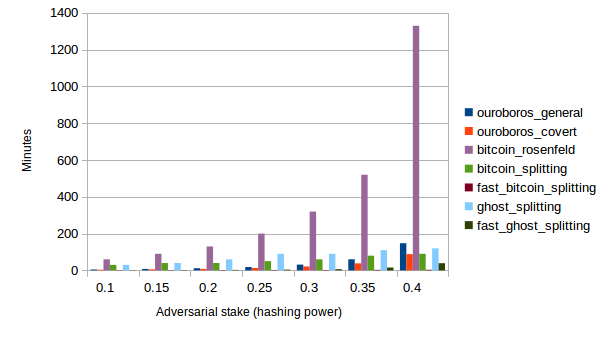
\includegraphics[width=0.85\textwidth]{time_comparison}
        \caption{Comparison of the expected confirmation period (in minutes) for different protocols and adversarial models.}
        \label{fig:time_comparison}
    \end{figure}
	
	\section{Conclusions}
	
	In this paper we presented the analysis of the different consensus protocols and adversarial models. The main goal was to compare the well-known proof-of-work protocol, that underlies Bitcoin, with the new proof-of-stake algorithm that was introduced in Ouroboros. We also had a look on the GHOST algorithm that is initially intended to improve Bitcoin consensus . As a measure of comparison we considered a transaction confirmation time that allows to be sure that the probability of a double-spend attack is less than 0.1\%.
	
	Together with the known results for Bitcoin we presented two models for two types of attacks on Ouroboros protocol (for the general and covert adversaries). The models allows to calculate exact number of slots needed to achieve the required level of security. It was shown that Ouroboros protocol allows to achieve the required security level with significantly shorter confirmation period compared to Bitcoin.
	
	We also examined a splitting attack that is targeted on the protocols with short block generation time. Our simulations showed the possibility of the attack for the Bitcoin and GHOST protocols with 10 min and 12.6 sec blocks. Not surprising that shorter blocks increase required number of blocks to confirm a transaction but, despite this, the overall confirmation time is significantly reduced due to fast blocks.
	    
	The obtained results allows to determine the security bounds for the Ouroboros system. It becomes extremely important for a real-world application because it will helps users to figure how long they should wait before accepting the transaction. We note that there are still some work to do on improvements of the presented models.
	
	
    \printbibliography
    
    \appendix
    
    \section{The Generalized Model of C. Pinzon et al.} \label{sec:generalized-model}
	
	The model proposed by C. Pinzon et al. \cite{PR16} generalizes the model of M. Rosenfeld by adding an extra parameter that represents time-advantage of an adversary.
	
	As in previous models, a successful double-spend attack consists of two constituents: the progress of an adversary during the confirmation period of \(m\) blocks and his ability to catch up from the deficit \(z = m - n\). The catch-up function is the same as originally proposed by S. Nakomoto. The improvement of this model lies in the modified progress function. It is represented as follows: \[P(q,m,n,t),\] where
	
	\(q\) -- fraction of hashing power that is possessed by an adversary (equivalent to the probability that he will find next block);
	
	\(m\) - number of blocks in the honest chain;
	
	\(n\) - number of blocks in the adversarial chain;
	
	\(t\) - time advantage of an adversary towards fraudulent block production.
	
	Basically the function \(P\) represents the probability of an adversary mining exactly \(n\) blocks once the honest network mines \(m\) blocks assuming that an adversary has been additionally mining secretly for \(t\) time units. While the first three parameters \((q,m,n)\) are well-known from the previous models, the time-advantage \(t\) is the new one. It represents an amount of time since the \(n^{th}\) block is found by an adversary until the \(m^{th}\) block is found by the honest network. This time period \(t\) potentially increases the probability of an adversary to find next block faster than the honest network thus giving him an advantage.
	
	In order to define the function \(P\), it is necessary to define the function \(a(q,t,k)\) that represents the probability to mine exactly \(k\) blocks during the time period \(t\) with a fraction \(q\) of hashing power (the proof could be found in the original paper \cite{PR16}):
	\[a(q,t,k) =
	    \left\{
            \begin{array}{ll}
                1 & if\  t = n = 0, \\
                0 & if\  t \leq 0, \\
                \frac{(qt)^k}{k!}e^{-qt} & otherwise. \\
            \end{array}
        \right.
	\]
	
	The function \(P\) can be defined as follows:
	\begin{equation}  \label{eq:pin_G_prog}
	    P(q,m,n,t) = \sum_{z=0}^{n}a(q,t,z)P_R(q,m,n-z).
	\end{equation}
	
	Note that in case of \(t=0\) the progress function \(P(q,m,n,t)\) is equivalent to the progress function presented by M. Rosenfeld \cite{R14}.
	
	It follows that the probability of a successful double-spend attack is equal to:
	\begin{equation}  \label{eq:pin_G_DS}
	    DS_G(q,K,n,t) = 1 - \sum_{z=0}^{K-n}P(q,K,z,t)(1 - C_R(q,K-n-z)),
	\end{equation}
	where
	
	\(q\) -- fraction of hashing power that is possessed by adversary (equivalent to the probability that he will find next block);
	
	\(K\) -- number of blocks in the honest chain;
	
	\(n\) -- number of blocks in the adversarial chain;
	
	\(t\) -- time advantage of the adversary;
	
	\(C_R(x,y)\) -- catch-up function as defined by M. Rosenfeld (eq. \ref{eq:ros_catchup}).
	
	Note that if the parameters \(t=0\) and \(n=1\) this model is equivalent to those represented by M. Rosenfeld \cite{R14}. 
	More information can be found in the original paper \cite{PR16}. 
	
	\section{The Time-based Model of C. Pinzon et al.} \label{sec:time-based-model}
	
	The second model presented by C. Pinzon et al. is completely different from those described in section \ref{sec:bitcoin_models}. In the time-based model the length of the valid and fraudulent chains are assumed to be equal. Instead, authors are focused on the time parameter \(t\) that represents time difference between the \(n^{th}\) block in adversarial and honest chains.
	
	We will not go deep into the details of this model, instead we will only present the final equation for calculating the probability of a double-spend attack. We refer an interested reader to the original paper \cite{PR16} to find more details about this model.
	
	The double-spend attack probability can be defined as the probability of having a time disadvantage \(t\) once the \(K+1'th\) block is mined, multiplied by the probability of catching up from that disadvantage:
	\begin{equation}  \label{eq:pin_T_DS}
	    DS_T(q,K,n_0,t_0) = \int_{-\infty}^{\infty} P(q,K+1,K-n_0+1,t)C_T(q,t-t_0)dt,
	\end{equation}
	where
	
	\(P\) -- progress function from the generalized model (eq. \ref{eq:pin_G_prog});
	
	\(C_T\) -- catch up function for the time-based model that is defined as follows:
	\[C_T(q,t) =
	    \left\{
            \begin{array}{ll}
                \frac{q}{p}e^{-(p-q)t} & if\ t > 0, \\
                1 & otherwise. \\
            \end{array}
        \right.
	\]
	
	The parameters of the eq. \ref{eq:pin_T_DS} are similar to the parameters of the eq. \ref{eq:pin_G_DS}.
	
\end{document}
	
